%-------------------------------- Configurações --------------------------------

\documentclass[
  a4paper,         % Tamanho do papel: A4
	abntfigtabnum,
  noindentfirst,
	normaltoc,
	pnumplain,
	notimes
	% capchap,
]{abnt}

\usepackage[utf8]{inputenc}
\usepackage[brazil]{babel}
\usepackage{url}
\usepackage{graphicx}
\usepackage{enumerate}
\usepackage[pdfborder={0 0 0}]{hyperref} % http://www.tug.org/applications/hyperref/manual.html
\usepackage[alf]{abntcite}
\usepackage{listings} % http://www.atscire.de/index.php?nav=products/listings2 http://linorg.usp.br/CTAN/macros/latex/contrib/listings/listings.pdf
\usepackage{textcomp}
\usepackage[usenames,dvipsnames]{xcolor} % http://en.wikibooks.org/wiki/LaTeX/Colors
\usepackage[algoruled,longend]{algorithm2e}
\usepackage{mathtools, mhsetup} % fórmulas matemáticas
\usepackage[usenames,dvipsnames]{pstricks} % gerar os gráficos
\usepackage{epsfig} % gerar os gráficos
\usepackage{float} % dependência do H para posição
\usepackage[all,cmtip]{xy}

\urlstyle{same} % http://en.wikibooks.org/wiki/LaTeX/Hyperlinks#Customization

%-------------------------------- Highligthing ---------------------------------

\lstset{
    language=C,
    basicstyle=\footnotesize\ttfamily,
    columns=flexible,
    numberbychapter=false,
    showstringspaces=false,
    tabsize=2,
    xleftmargin=17pt,
    framexleftmargin=17pt,
    framexrightmargin=5pt,
    framexbottommargin=4pt,
    numbers=left,
    numberstyle=\scriptsize\ttfamily\color{Gray},
    emphstyle=\color{OrangeRed},
    commentstyle=\color{Gray}\textit,
    stringstyle=\textit,
    keywordstyle=\textbf,
    morekeywords={@self, @caller, @const, @local},
    % emph={[2]Funcionalidade, Como},
    % emphstyle=[2]\color{MidnightBlue},
}

\usepackage{caption}
\DeclareCaptionFont{white}{\color{white}\footnotesize\bfseries}
\DeclareCaptionFormat{listing}{\colorbox{BrickRed}{\parbox{\textwidth}{#1#2#3}}}
\captionsetup[lstlisting]{format=listing,labelfont=white,textfont=white}

% Renomear listing e listings -> código e códigos
\renewcommand*\lstlistingname{Código}
\renewcommand*\lstlistlistingname{Lista de Códigos}

%--------------------------------- Informações ---------------------------------
\newcommand{\meutitulo}{A Programação Linear aplicada ao reconhecimento de expressões faciais, com ênfase no método Simplex Revisado}
\begin{document}

\titulo{\meutitulo}
\autor{Renata Gomes Cordeiro}
\instituicao{Universidade Estadual do Norte Fluminense Darcy Ribeiro}
\orientador[Tutor: ]{Fermín Alfredo Tang Montané.}
\comentario{Monografia apresentada ao Curso de Graduação em Ciência da
Computação da Universidade Estadual do Norte Fluminense Darcy Ribeiro como
requisito para obtenção do título de Bacharel em Ciência da Computação, sob
orientação do Profº. Fermín Alfredo Tang Montané.}
\local{Campos dos Goytacazes/RJ}
\data{2012}

\graphicspath{{graficos/}}
\capa
\folhaderosto

\sumario

\chapter{Introdução}

\section{Considerações Iniciais}
A programação linear é uma das disciplinas que compõem a programação matemática e constitui um dos pilares da pesquisa operacional. As aplicações da programação linear estão presentes em diversos setores, tais como nas indústrias, nos transportes, na saúde, na educação, na administração pública. etc.  Além disso, a resolução de problemas de programação linear (PPL) é requerida em outras disciplinas da programação matemática como programação inteira e programação não-linear, onde é comum a resolução de vários PPL de forma repetida.

O método simplex proposto por \citeonline{Dan} é um dos métodos mais conhecidos e eficientes para resolver problemas de programação linear. Trata-se de um dos poucos algoritmos que foi implantado comercialmente há mais de 40 anos. Atualmente, está presente em softwares comerciais tais como CPLEX e LINGO. Um método alternativo, teoricamente superior ao método simplex, é o método dos pontos interiores, proposto por \citeonline{Karmarkar}. Na prática, tanto o método simplex, quanto o método dos pontos interiores competem até hoje.  
(FALAR O QUE É O SIMPLEX REVISADO)
O presente trabalho, por opção, é focado especificamente no método simplex revisado. Busca-se o desenvolvimento de um aplicativo capaz de resolver problemas de programação linear utilizando o método simplex revisado. Acredita-se que a importância desse trabalho se deve ao intuito de explorar o conhecimento a respeito do método, e acima disso o desenvolvimento de uma ferramenta gratuita que proporcione ao usuário uma interface intuitiva e de fácil entendimento.

\section{Objetivos e justificativas}
O objetivo do presente trabalho é o estudo da utilização da programação linear, mais especificamente o método simplex, no reconhecimento de expressões faciais. 

Através desse estudo deve ser possível verificar a eficiência da programação linear nesse tipo de aplicação da computação gráfica. Além disso, devem ser realizadas duas comparações do resultado final obtido, do ponto de vista computacional: a utilização da programação linear e outro método mais comumente utilizado na computação gráfica; e a utilização de uma biblioteca desenvolvida e uma implementação do modelo de progra,ação linear utlizando o softwrae Cplex.

A programação linear possui aplicações em diversas áreas, como: indústria, produção, saúde e computação gráfica. Porém é um método mais comumente utilizado na engenharia de produção em problemas como: alocação de recursos e planejamento de produção. O presente trabalho justifica-se pelo fato de querer abordar uma aplicação prática dentro da computação, mais especificamente na computação gráfica, onde a aplicação da programação linear não é tão explorada quanto na engenharia de produção.

\section{Metodologia}
Para o cumprimento do obejtivo final, o trabalho é composto por algumas etapas:

\begin{itemize} 
\item O estudo do método simplex revisado, suas características, vantagens do ponto de vista computacional e suas variantes.
\item O desenvolvimento da biblioteca para resolução de problemas de programação linear
\item A implementação do modelo do problema de programação linear no software Cplex
\item Aplicação da biblioteca e da implementação feita no Cplex em alguma aplicação de computação gráfica para reconhecimento de expressões faciais.
\end{itemize}

Para a reralização desta última etapa, espera-se, através de pesquisas encontrar uma aplicação pronta que realize o reconhecimento de expressões faciais que deverá ser utilizada. Porém ao invés de realizar o processamento utilizando o método já incorporado à aplicação, o método simplex será utilizado. Caso não seja encontrada uma aplicação de reconhecimento de expressão facial, que torne viável a substituição do método utilizado, uma ferramenta de forneça essa funcionalidade será desenvolvida.

\section{Estrutura do trabalho} (COLOCAR A ESTRUTURA COMPLETA DA  MONOGRAFIA)
O presente trabalho apresenta a seguinte estrutura: o capítulo 2 apresenta uma descrição do problema geral de programação linear, os principais métodos de solução, algumas aplicações práticas e as ferramentas computacionais disponíveis. 

\chapter{Referencial teórico}
Este capítulo apresenta um revisão teórica sobre as principais metodologias utilizadas nesse trabalho: programação linear, métodos de classificação e métodos de validação. Também é apresentada uma revisão de trabalhos sobre classificação de dados.  

\section{A programação linear}
Na pesquisa operacional, a programação linear é uma das técnicas mais utilizadas para resolver problemas de otimização. Os problemas de programação linear geralmente buscam a distribuição eficiente de recursos limitados para atender um determinado objetivo, por isso suas aplicações estão presentes em diversas áreas como computação, administração, indústria e transporte \cite{Engecom}.

Um problema de programação linear é expresso através de um modelo composto por equações e inequações lineares. Esse tipo de problema busca a distribuição eficiente de recursos com restrições para alcançar um objetivo, em geral, maximizar lucros ou minimizar custos. Em um problema de programação linear esse objetivo é expresso através de uma equação linear denominada função objetivo. Para a formulação do problema, é necessário também definir os recursos necessários e em que proporção são requeridos. Essas informações são expressas em equações ou inequações lineares, uma para cada recurso. Esse conjunto de equações ou inequações é denominado restrições do modelo \cite{Engecom}.

\section{Descrição do problema de programação linear}
O modelo de um problema de programação linear é apresentado em uma das formas a seguir:
\noindent
\underline{\bf Modelo 1}
\begin{eqnarray}
    Max\ z = c^{T}x \label{eq:obj1}
\\s.a.\left\{\begin{matrix}
Ax\leq b\\*x\geq 0
\end{matrix}\right.\label{eq:rest1}
\end{eqnarray}
\\
\noindent
\underline{\bf Modelo 2}
\begin{eqnarray}
Min\ z = c^{T}x \label{eq:obj2}
\\*s.a.\left\{\begin{matrix}
Ax\geq  b\\*x\geq 0 
\end{matrix}\right. \label{eq:rest2}
\end{eqnarray}

Nos Modelos 1 e 2 as equações \ref{eq:obj1} e \ref{eq:obj2} representam as funções objetivo e as inequações \ref{eq:rest1} e \ref{eq:rest2} representam as restrições.
Onde, 
\begin{itemize}
\item \textbf {$x$} é o vetor com as variáveis do modelo
\item \textbf {$c$} é o vetor de coeficientes da função objetivo
\item \textbf {$z$} é o valor da função objetivo
\item \textbf {$A$} é a matriz com as constantes das restrições
\item \textbf {$b$} é o vetor com os valores limites das restrições
\end{itemize}

Sendo que c, A e b são dados conhecidos.

A seguir é apresentado um exemplo de aplicação da programação linear no contexto da otimização da produção. Uma empresa, que fabrica vários produtos, deseja maximizar o lucro na venda de dois desses produtos.
A produção é feita em três setores diferentes e está sujeita a restrições de tempo disponível para a produção em cada setor.
O problema pode ser representado pelo seguinte modelo de programação linear com duas variáveis\cite{Hillier}.

\begin{eqnarray}
Maximize\ z=3x_{1}+5x_{2}\label{eq2:eq1}\\ 
Sujeito\ a \nonumber \\ 
1x_{1}\leq 4 \label{eq2:eq2} \\  
2x_{2}\leq 12 \label{eq2:eq3} \\ 
3x_{1}+2x_{2}\leq 18 \label{eq2:eq4}\\ 
x_{1}\geq 0, x_{2}\geq 0 \label{eq2:eq5}
\end{eqnarray}

Onde, 
\begin{itemize}
\item \textbf {$x_{1}$} representa a quantidade do produto 1 produzido em uma semana.
\item \textbf {$x_{2}$} representa a quantidade do produto 2 produzido em uma semana.
\item \textbf {$z$} representa o lucro total por semana de produção desses dois produtos (em milhões de dólares), sendo o lucro do produto 1 de 3 milhões e o do produto 2 de 5 milhões.
\end{itemize}

E as restrições representam as restrições de tempo de cada setor que compõe o processo de produção.
\begin{itemize}
\item A equação \ref{eq2:eq2} garante que, durante o processo de produção, cada produto 1 necessita de 1 hora no setor 1, e o setor só tem disponível 4 horas por semana.
\item A equação \ref{eq2:eq3} garante que, durante o processo de produção, cada produto 2 necessita de 2 horas no setor 2, e o setor só tem disponível 12 horas por semana.
\item A equação \ref{eq2:eq4} garante que, durante o processo de produção, cada produto 1 necessita de 3 horas no setor 3, e cada produto 2 necessita de 2 horas no setor 3, e o setor só tem disponível 18 horas por semana.
\item A equação \ref{eq2:eq5} garante que, os dois produtos devem ser produzidos.
\end{itemize}

Um problema de programação linear com até três variáveis pode ser representado graficamente utilizando três eixos cartesianos. Os problemas com duas variáveis podem ainda ser facilmente resolvidos por meio da representação gráfica \cite{Passos}. 

A seguir, o problema exemplo é apresentado graficamente. Apesar de, na prática os modelos de programação linear possuírem um número de variáveis muito maior que dois ou três, a visualização gráfica do modelo, mesmo que simples, contribui para o entendimento dos métodos de resolução apresentados no capítulo a seguir.
\begin{center}
	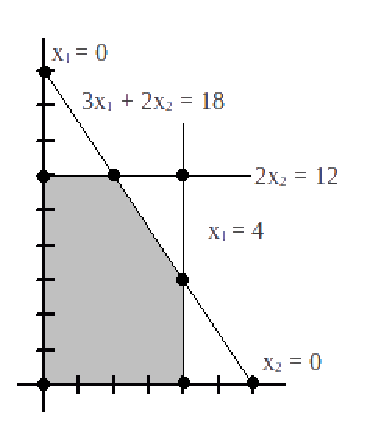
\includegraphics[scale=1.0]{graficos/simplex_graf}
	\captionof{figure}{Representação gráfica do modelo de programação linear de duas variáveis}
	\label{img:simplex_grafico}
\end{center}


Onde cada reta representa uma restrição do modelo, e a área cinza representa a região viável, ou seja, nessa área estão contidas os valores viáveis de $x_{1}$ e $x_{2}$ para a maximização do lucro.

Os métodos para resolução de problemas de programação linear buscam esses valores de $x_{1}$ e $x_{2}$  para a determinação da solução ótima.

\section{Aplicações utilizando programação linear}
Um problema de programação linear, como já dito anteriormente, busca um resultado ótimo sujeito a restrições, com utilização em diversas áreas.

A programação linear se aplica na área da saúde, como demonstrado por \citeonline{Alterovitz-saude} em seu trabalho. Em um determinado tipo de tratamento de câncer são inseridos cateteres na área afetada para introduzir o medicamento necessário, porém o medicamento acaba afetando células saudáveis além das cancerígenas. Como os problemas de programação linear podem ser resolvidos como problemas determinísticos e com solução exata, \citeonline{Alterovitz-saude} propõe a formulação de um problema de otimização para determinar o tempo de permanência dos cateteres, minimizando os desvios em relação a quantidade da dose necessitada pelo paciente através da minimização de custos atribuídos. Nos testes realizados, foi obtida uma melhoria nos desvios em relação a quantidade da dose necessitada pelo paciente mas clinicamente os resultados obtidos não mostraram uma vantagem significativa em relação ao método atualmente utilizado.

Em \citeonline{Moreira2003Saude} modelos de programação linear foram desenvolvidos para duas aplicações relacionadas a área da saúde. Em um dos modelos busca-se a formulação de uma dieta com custo mínimo, considerando as restrições alimentares e os nutrientes essenciais em uma dieta. Um segundo modelo visa analisar intervenções médicas que buscam maximizar os anos de vida de pacientes considerando uma população, como restrições são utilizados os custos e o número de visitas médicas. Para a resolução dos modelos foi utilizado o método simplex. O autor considerou a programação linear como um instrumento útil na tomada de decisões na área da saúde, considerando a importância da substituição de métodos tradicionais baseados no bom senso e tentativa de acerto por métodos com soluções otimizadas.

Nos trabalhos de \citeonline{Alterovitz-saude} e \citeonline{Moreira2003Saude} foi exemplificado como a programação pode ser útil e importante na área da saúde. No primeiro trabalho apesar de não demonstrar uma melhoria no resultado geral, foi comprovada a equivalência dos resultados com o método probabilístico atualmente utilizado. Em \citeonline{Moreira2003Saude} apesar dos dados utilizados serem reduzidos e uma dieta real possuir mais restrições que as propostas no trabalho, o autor demonstrou a aplicabilidade da programação linear em duas situações da área da saúde.

Em \citeonline{Possami2011Logistica} a programação linear foi utilizada na resolução de um problema abrangendo o transporte, o processamento e a estocagem de fumo, buscando como objetivo a minimização dos custos. O modelo proposto foi composto por 650 variáveis e 150 restrições. A partir do resultado obtido foi possível determinar parâmetros desde o transporte da matéria bruta, estocagem até a venda do produto.

Dentre as aplicações mais conhecidas da programação linear, encontram-se os problemas de planejamento de produção e controle de estoque, assuntos relacionados a engenharia de produção, como no trabalho de \citeonline{Possami2011Logistica}. A partir desse trabalho tem-se o exemplo de como os resultados extraídos de um modelo de programação linear podem ser determinantes no sucesso de um processo de produção.

Em seu trabalho \citeonline{Krukoski2010Economia} propõe a utilização da programação linear na economia. Considerando que os investimentos em ações estão cada vez mais acessíveis para pequenos investidores, o autor propõe um modelo de programação linear na determinação de uma operação de compra ou venda que maximize o lucro e baseando-se também nos riscos. Os resultados obtidos em sua maioria foram positivos e lucrativos, apesar de, de acordo com o autor, algumas operações obtidas nos resultados serem pouco aplicáveis se comparadas às atitudes rotineiras dos investidores.

No trabalho proposto por \cite{Krukoski2010Economia} foi apresentada uma aplicação que pode auxiliar na tomada de decisões na área da economia. Os bons resultados mostram que a programação linear, como método determinístico, pode ser empregada mesmo em problemas que estão mais relacionados a métodos probabilísticos, como é o caso dos investimentos em ações.

A programação linear além de estar presente, é fundamental em diversas áreas, tornando-se uma ferramenta de apoio a decisão e contribuindo para o sucesso de projetos nas áreas em que se aplica.

\section{Métodos de classificação}
Em problemas de classificação, dado um conjunto de dados dividido entre conjunto de treinamento e conjunto de teste, onde, no conjunto de treinamento cada subconjunto pertence a um entre \textit{n} padrões, o objetivo é que a partir de um dado do conjunto de teste o método de classificação retorne a qual dos \textit{n} padrões esse dado pertence. A seguir são apresentados alguns dos métodos de classificação mais citados na literatura. 

\subsection{\it Support Vector Machines}
\textit{Support Vector Machines} (SVM) ou Máquinas de vetores de suporte têm a capacidade de gerar classificadores na etapa de treinamento e de classificar os dados na etapa de teste de acordo com os classificadores gerados. Considerando um problema de classificação com dois padrões, uma SVM irá determinar um plano que separe os pontos desses dois padrões, de forma que a distância entre o hiperplano e os pontos seja a máxima possível. Os pontos de cada padrão utilizados como referência são denominados vetores de suporte.
No caso de conjuntos linearmente inseparáveis, é utilizada um função denominada Kernel. Essa função é responsável por elevar a dimensão espacial a fim de que os pontos se tornem linearmente separáveis. Portanto para a obtenção de um classificador utilizando SVM é necessária a escolha de uma função kernel e os parâmetros dessa função. Essa escolha influencia diretamente no desempenho do classificador\cite{Gunn98SVM}\cite{Reffson02SVM}.

No caso em que o número de padrões é maior que dois, duas abordagens podem ser utilizadas com as SVM \cite{Lorena03SVM}:
\begin{itemize}
\item{\textbf{Um contra todos:} }Nessa abordagem, para \textit{k} padrões são geradas \textit{k} SVM. Na criação das SVM, é gerado um hiperplano que separa 1 padrão dos \textit{k}-1 padrões. Na determinação do padrão de um dado x, o padrão é aquele que, entre as \textit{k} SVM obteve x do lado do hiperplano onde se encontrava o padrão separado dos demais.  
\item{\textbf{Todos contra um:} }Nessa abordagem os padrões são agrupados em pares e uma SVM é gerada para cada par. Um esquema de votação deve ser utilizado para determinar o padrão de uma instância, que deve ser analisada a partir de cada SVM e cada SVM retorna um padrão possível. O padrão que obtiver mais pontos da instância é a classe atribuída.
\end{itemize}

\subsection{\it Naive Bayes}
Na metodologia \textit{Naive Bayes} as características do dado a ser classificado são analisadas de forma independente. O vetor de características é formado pela número de vezes que cada característica ocorre no dado caracterizado. A probabilidade de uma instância pertencer a um determinado padrão é dada por uma probabilidade inicial, baseada na quantidade total de dados, e pelas probabilidades das ocorrências das características \cite{McCallum98Bayes} \\
\cite{Langley92Bayes}. %Essa abordagem é mais comumente utilizada na área de mineração de dados, onde dada uma palavra busca-se o melhor texto baseado na quantidade de vezes que a palavra aparece da palavra no textos utilizados no treinamento% \

\subsection{\textit{k}- nearest neighbor}
Nesse método a classificação é feita pela similaridade da instância a ser classificada com um dado ou vetor utilizado no treinamento, a classe do dado utilizado no treinamento é então atribuída a instância com padrão inicialmente desconhecido. As etapas desse método consistem em utilizar um parâmetro para medir a semelhança ou a distância do dado a ser classificado em relação a cada um dos dados utilizados no treinamento. Os \textit{k} vetores mais similares ou mais próximos são selecionados e entre o padrão mais frequente é atribuído ao dado inicialmente desconhecido. Apesar de ser considerado um método simples, sua dificuldade está em definir os parâmetros ou a métrica que definirá a semelhança ou distância entre os dados\cite{Chagas09KNN}.

\subsection{Redes Neurais Artificias}
Em seu trabalho  \citeonline{Morais2010RNA} define Redes Neurais Artificiais (RNA) como sistemas paralelos e distribuídos compostos por unidades de processamento simples (neurônios) interligadas por conexões, esses neurônios calculam determinadas funções matemáticas. Na fase de treinamento ou aprendizagem "um conjunto de exemplos é apresentado a rede que extrai automaticamente características necessárias para representar a informação fornecida" \cite{Morais2010RNA}.
Uma rede neural pode receber como entrada, na etapa de treinamento, um conjunto de vetores com seus respectivos padrões. Ao submeter como entrada um vetor com padrão desconhecido a rede neural deve classificar esse vetor. A vantagem desse método é que uma rede pode construir fronteiras não lineares entre padrões, o que pode ser muito vantajoso em problemas complexos de classificação. Existem vários modelos de redes neurais que possibilitam o reconhecimento de padrões, entre eles: Perceptron de Camada Simples, Perceptron de Múltiplas e Redes de Kohonen \cite{ZubenRNA2}.

\section{Aplicações em classificação de dados}
Em seu trabalho \citeonline{Reffson02SVM} busca o classificação de impressões digitais em 5 padrões. Esse tipo de classificação tem o propósito de gerenciar grandes bancos de dados de impressões digitais e acelerar o processo de identificação. Foi utilizado um banco contendo 4000 imagens igualmente distribuídas entre os cinco padrões. O autor dividiu o banco em dois grupos, utilizando um para treinamento e outro para teste. Após a extração das características das imagens, Máquinas de Vetores de Suporte foram utilizadas na classificação. Na abordagem todos contra um foi obtida uma média de precisão de 91,18\%, já na abordagem um contra todos a precisão na classificação das impressões foi de 90,43\%.

\citeonline{Chagas09KNN} apresentou uma técnica para a classificação de textos, uma atividade importante em aplicações como bibliotecas digitais e em outras que em geral buscam a organização de documentos disponíveis no formato digital. O autor propôs variações no método \textit{k near neighbor} a fim de  aprimorar a escolha dos textos, utilizados no treinamento, mais próximos ao texto que precisa ser classificado. Nos testes feitos com três coleções de textos, as médias de acertos na classificação obtidas foram acima de 90\% em duas coleções, e próxima a 70\% na terceira.

No trabalho de \citeonline{sbai2003RNALaranjas} uma rede neural artificial foi utilizada na classificação de laranjas através de imagens. Os autores consideraram que apesar da automação de muitos setores industriais, em um sistema de produção, as frutas consideradas boas, são selecionadas através de inspeção visual humana. A principal característica utilizada foi a cor, que pode classificar a fruta em cinco padrões. No trabalho ficou comprovada a aplicabilidade do método para o domínio proposto que era classificar as frutas de acordo com a cor.

\section{Métodos de validação da metodologia}
Uma metodologia de classificação pode ser verificado em relação a sua acurácia a partir de um conjunto de dados ou a sua performance em relação a outros métodos classificadores. Algumas técnicas utilizadas com esse intuito serão apresentadas a seguir. No presente trabalho a técnica Cross Validation é utilizada com o objetivo de verificar a acurácia, nesse caso, da metodologia utilizada na classificação de dados.

A seguir são apresentadas as três técnicas mais comumente encontradas na bibliografia com suas ventagens e desvantagens:

\subsection{\textit{Handout}}
Esse é um método simples, onde os dados são divididos em 2 grupos mutuamente exclusivos, sendo um grupo utilizado para treino e o outro para teste. Em geral 2/3 dos dados são utilizados no treinamento e 1/3 na etapa de testes. Os dois grupos devem conter dados suficientes de todos os padrões, nesse caso, suficientes para que o resultado final não seja comprometido pela falta de dados, de um determinado padrão, no grupo da etapa de treino e nem no grupo de testes. Apesar de ser um método de fácil implementação, a divisão entre conjunto de treinamento e teste deve ser bem estudada de forma que todos os padrões estejam bem representados nos dois grupos, por isso é um método recomendável quando o conjunto de dados possui um grande número de representações de cada padrão \cite{Kohavi95Cross} \cite{Baldisserotto05Validacao}.

\subsection {\textit{Cross Validation}}
Nesse método, o conjunto de dados também é dividido em conjunto de treinamento e de teste, porém esses dois grupos variam a cada rodada de teste. O tipo de \textit{cross validation} mais comumente utilizado é o \textit{k-fold cross validation}, onde os dados são divididos em k conjuntos mutuamente exclusivos e as etapas de treinamento e teste são realizadas k vezes, de forma que a cada rodada um conjunto diferente é utilizado como teste e os outros k-1 conjuntos são utilizados para treinamento. Esse método é recomendável quando o conjunto de dados não é tão grande, pois não existe uma  preocupação de quais dados separar para teste e quais separar para treinamento, já que ao final da execução do método todos o dados terão participado dos conjuntos de treinamento e teste \cite{Kohavi95Cross} \cite{Baldisserotto05Validacao}.

\subsection{\textit{Leave-one-out}}
Nessa técnica, do conjunto com o número total de dados n, são realizadas n rodadas de treinamento e teste, sendo que a cada rodada n-1 dados são utilizados para teste e o dados restantes são utilizados para treinamento. Pelas suas características, esse é um método recomendável para conjuntos de dados pequenos já que a quantidade de rodadas de treinamento e teste é igual a quantidade de dados o que o torna um método com alto custo computacional \cite{Kohavi95Cross} \cite{Baldisserotto05Validacao}.

\chapter{Aplicação da programação linear no reconhecimento de padrões}
Na tarefa onde o obejtivo é a separação de dois ou mais conjuntos de pontos, sendo que cada conjunto representa um padrão, busca-se um método para que essa separação seja obtida com resultado ótimo. Cada conjunto é o resultado de um conjunto de pontos e cada ponto é representado por um vetor de características.
Em \cite{Bennett92robustlinear} é proposto um modelo de programação linear capaz de um gerar um hiperplano, que separa dois conjuntos de pontos, minimizando a soma dos pontos que permaneceram do lado errado do hiperplano. Dessa forma o modelo é capaz de gerar um hiperplano separador para pontos linearmente separáveis e para conjutnos linearmente inseparáveis, o modelo gera o melhor hiperplano de forma que essa média calculada seja mínima. Na figura abaixo estão ilustrados os casos de dois conjuntos linearmente separáveis e dois conjuntos linearmente inseparáveis.
 
\begin{figure}
\centering
\subfigure[]{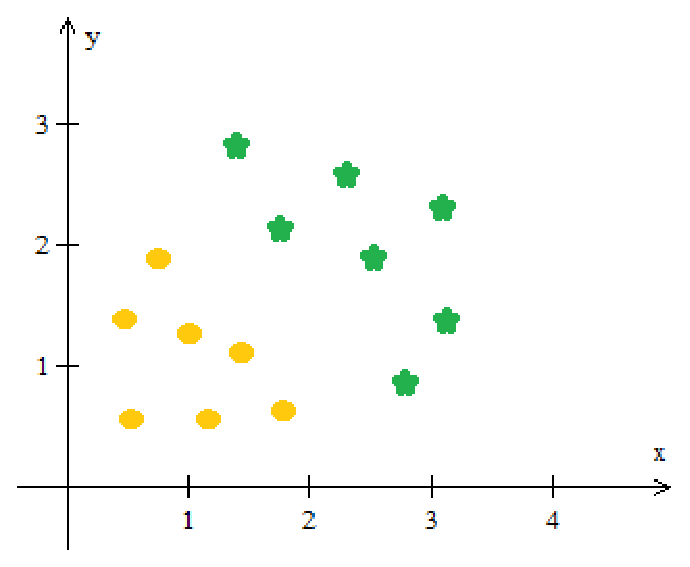
\includegraphics[scale=0.5]{graficos/linear_sepa}\label{fig1}}
\qquad
\subfigure[]{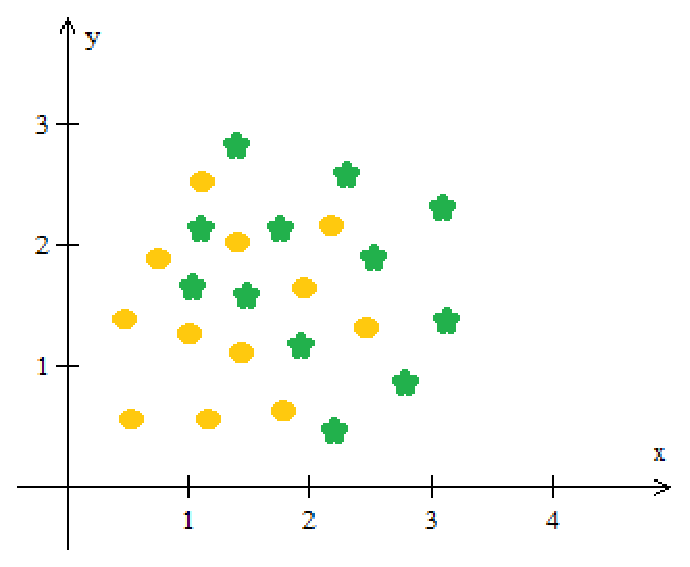
\includegraphics[scale=0.5]{graficos/linear_insepa}\label{fig2}}
\label{img:linear_sepa}
\caption{Em \ref{fig1} são apresentados dois conjuntos linearmente separáveis e em \ref{fig2} são apresentados dois conjuntos linearmente inseparáveis}
\end{figure}

É possível observar que na figura \ref{fig1} podem ser tratadas inúmeras retas seprando os dois conjuntos de pontos. Já na figura \ref{fig2} o modelo de programação linear poderá definir a melhor reta possível para separar os pontos.

A proposta do modelo e separa dois conjuntos de pontos, porém também pode ser utlizado em problemas onde busca-se a separação de múltiplos padrões. O presente trabalho foca nessa última abordagem, em todos os testes realizados o número de conjutnso de pontos é igual ou maior que três.

\section{O modelo}
Considerando dois conjuntos, no espaço n-dimensional $ R^{n} $, sendo o conjunto A representado pela matriz m x n, e o conjunto B representado pela matriz k x n. Contextualizando, k e m são as quantidades de pontos em cada conjunto, e n é a quantidade de características. O modelo gera um hiperplano que separa os pontos dos dois conjuntos. De forma que os m pontos do conjunto A fiquem de um lado do hiperplano e os k pontos do conjunto B fiquem do outro lado do hiperplano. Na figura abaixo o modelo é apresentado. E a seguir é apresentado de forma mais detalhada.

$$\min_{\omega ,\gamma ,y,z}\frac{e^{T}y}{m}+\frac{e^{T}z}{k}$$
$$s.a.\left\{\begin{matrix}-A\omega +e\gamma+e\leq y\\B\omega -e\gamma+e\leq  z\\ y\geq 0,y\geq 0\end{matrix}\right.$$

O modelo determina o hiperplano:
$$ x\omega = \gamma $$
Onde,  é $\omega$ o vetor normal ao hiperplano e $\gamma$ é um escalar. De forma que:
$$A\omega \geq e\gamma$$
e
$$B\omega \leq e\gamma$$
Onde e é um vetor de 1’s com dimensão m para o conjunto A e k para o conjunto B.
Para conjuntos linearmente separáveis torna-se fácil traçar um hiperplano separador, porém para conjuntos linearmente inseparáveis é necessária uma estratégia para que o hiperplano separador seja ótimo.
O modelo busca o melhor hiperplano, para isso gera dois hiperplanos limites somando 1 unidade a equação do hiperplano separador:
$$A\omega \geq e\gamma + e$$
e
$$B\omega \leq e\gamma - e$$
De forma que o hiperplano separador fica localizado exatamente entre esses dois hiperplanos limites.
Detalhando o modelo de acordo com \citeonline{Eberson10LPseparaPontos}, considerando x como um vetor em $ R^{n} $, definimos:

$1.\ \ (x_{i})_{+} = \max_{i=1,2,...,n}{\left \{x_{i},0  \right \}}$

$2.\ \ \left \| xx \right \|_{1} = \sum_{i=1}^{n}\left | x_{i} \right |$

Podemos escrever o problema de minimização com norma da seguinte forma:

$$\min_{\omega ,\gamma }\frac{1}{m}\left \| \left ( -A\omega + e\gamma  + e \right )_{+} \right \|_{1} + \frac{1}{k}\left \| \left ( B\omega - e\gamma + e  \right )_{+} \right \|_{1}$$

Seja $g:R^{n} \mapsto R^{m} , h:R^{n} \mapsto R^{k}$ e S um subconjunto de $R^{n}$ . Os problemas abaixo possuem soluções idênticas:

$$\min_{x\in S}\left \| g(x)_{+} \right \|_{1} + \left \| h(x)_{+} \right \|_{1}$$


$$\min_{x\in S} e^{t}y + e^{t}z\\$$
$$ s.a.\left\{\begin{matrix}y\geq g(x)\\ z\geq h(x)\\ y\geq 0, z\geq0\end{matrix}\right.$$

Como $g(x)_{+}\geq g(x)$ e $h(x)_{+}\geq h(x)$ podemos observar que os valores ótimos de y e z podem der dados pelas igualdades $y=g(x)_{+}$ e $z=h(x)_{+}$.

A partir do problema de minimização temos o problema de programação linear equivalente:

$\min_{\omega ,\gamma ,y,z}\frac{e^{T}y}{m}+\frac{e^{T}z}{k} \; \; \; \; (a)\\
s.a.\left\{\begin{matrix}-A\omega +e\gamma+e\leq y\; \; (b)\\B\omega -e\gamma+e\leq  z\; \; (c)\\ y\geq 0,y\geq 0\; \; (d)\end{matrix}\right.$

\underline{Dados do Modelo}:
\begin{itemize}
\item{m}: quantidade de imagens no conjunto correspondente a primeira expressão facial;
\item{k}: quantidade de imagens no conjunto correspondente a segunda expressão facial;
\item{A}: Matriz contendo o conjunto de vetores de caraterísticas das imagens correspondentes à primeira expressão facial;
\item{B}: Matriz contendo o conjunto de vetores de caraterísticas das imagens correspondentes à segunda expressão facial;
\item{e}:  vetor coluna unitário;
\end{itemize}

\underline{Variáveis do Modelo}:
\begin{itemize}
\item{$\omega$}: coeficientes do hiperplano que separa os conjuntos de imagens em dois grupos;
\item{$\gamma$}: constante do hiperplano que separa os conjuntos de imagens em dois grupos;
\item{y}: vetor contendo as distâncias de cada imagem do conjunto A ao hiperplano separador mais um;
\item{z}: vetor contendo as distâncias de cada imagem do conjunto B ao hiperplano separador mais um.
\end{itemize}

\underline{Formulação Matemática}:

	A função objetivo (a) procura minimizar a somas das médias das distâncias das imagens de ambos conjuntos. A restrição (b) exige que os pontos se encontrem necessariamente abaixo do hiperplano separador mais uma constante unitária.  A restrição (c) é análoga a restrição (b) aplicada as imagens da segunda expressão facial. As equações em (d) definem a natureza das variáveis do modelo, como sendo não negativas.

\section{Exemplo Ilustrativo do Modelo Classificador}
Para ilustrar o modelo vamos considerar dois exemplos em $R^{2}$ \cite{Bennett92robustlinear} de forma que a ilustração gráfica fique mais facilmente compreensível.
\begin{itemize}
\item Exemplo1:

Considerando as matrizes a seguir:
$$A=\begin{bmatrix}1 & 1\\ 1 & 2\\ 1 & 3\\ 2 & 1\\ 2 & 2\\ 2 & 3\\ 2 & 4\\ 3 & 3\\ 3 & 4\end{bmatrix}
B=\begin{bmatrix}4 & 1\\ 4 & 2\\ 4 & 3\\ 5 & 2\\ 5 & 3\\ 5 & 4\\ 6 & 2\end{bmatrix}$$

Nesse caso, temos: m = 9 (quantidade de pontos da matriz A) e k = 7 (quantidade de pontos da matriz B).  Submetendo as matrizes ao modelo temos:
\begin{itemize}
\item[$\ast$] Valor da função objetivo = 0
\item[$\ast$] $\omega$ = [-2  0]
\item[$\ast$] $\gamma$ = -7
\item[$\ast$] y = [0 0 0 0 0 0 0 0 0]
\item[$\ast$] z = [0 0 0 0 0 0 0]
\end{itemize}
Como o valor da função objetivo depende dos vetores y e z, podemos notar que o valor 0 indica que os conjuntos A e B são linearmente separáveis. A seguir é apresentada a representação gráfica dos pontos e das retas geradas pelo modelo.

\begin{center}
	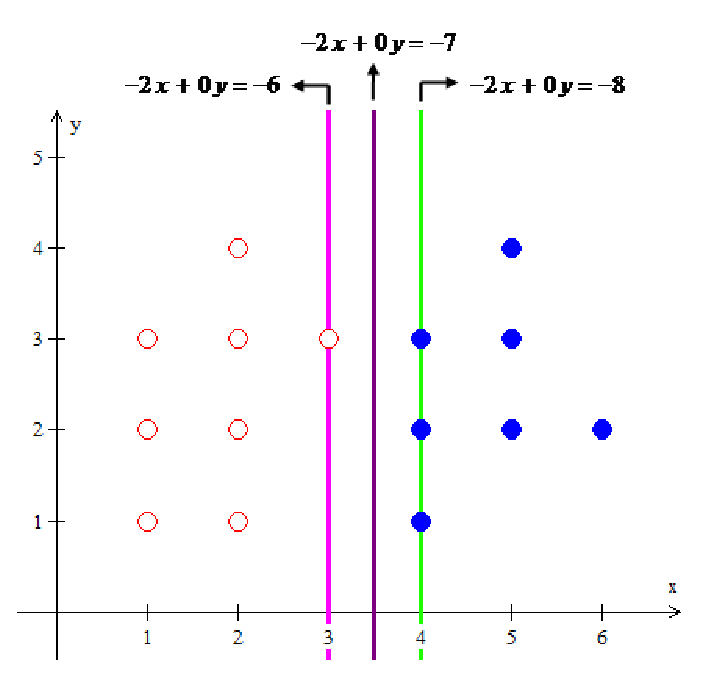
\includegraphics[scale=0.5]{graficos/exemplo2}
	\captionof{figure}{Representação ilustrativa do exemplo 1}
	\label{img:ex1}
\end{center}

A partir da representação gráfica podemos perceber que a reta separadora $-2x + 0y = -7$ se localizou exatamente no meio entre os dois conjuntos com o auxílio das duas retas: $-2x + 0y = -6$ e $-2x + 0y = -8$.

\item Exemplo2:
Vamos  considerar agora as matrizes:
$$A=\begin{bmatrix}3 & 4\\ 4.3 & 4.5\\ 4.5 & 2\\ 3 & 5.5\end{bmatrix}
B=\begin{bmatrix}4 & 2\\ 4.5 & 3.5\\ 5 & 3\end{bmatrix}$$

Neste exemplo temos: m = 4 e k = 3. De acordo com o modelo, temos os seguintes valores:
\begin{itemize}
\item[$\ast$] Valor da função objetivo = 0.92
\item[$\ast$] $\omega$ = [-0.91  0.91]
\item[$\ast$] $\gamma$ = -0.82
\item[$\ast$] y = [0 0 2.46 0]
\item[$\ast$] z = [0 0.91 0]
\end{itemize}

Com o valor da função objetivo diferente de zero, temos dois conjuntos linearmente inseparáveis, como ilustrado na figura a seguir.

\begin{center}
	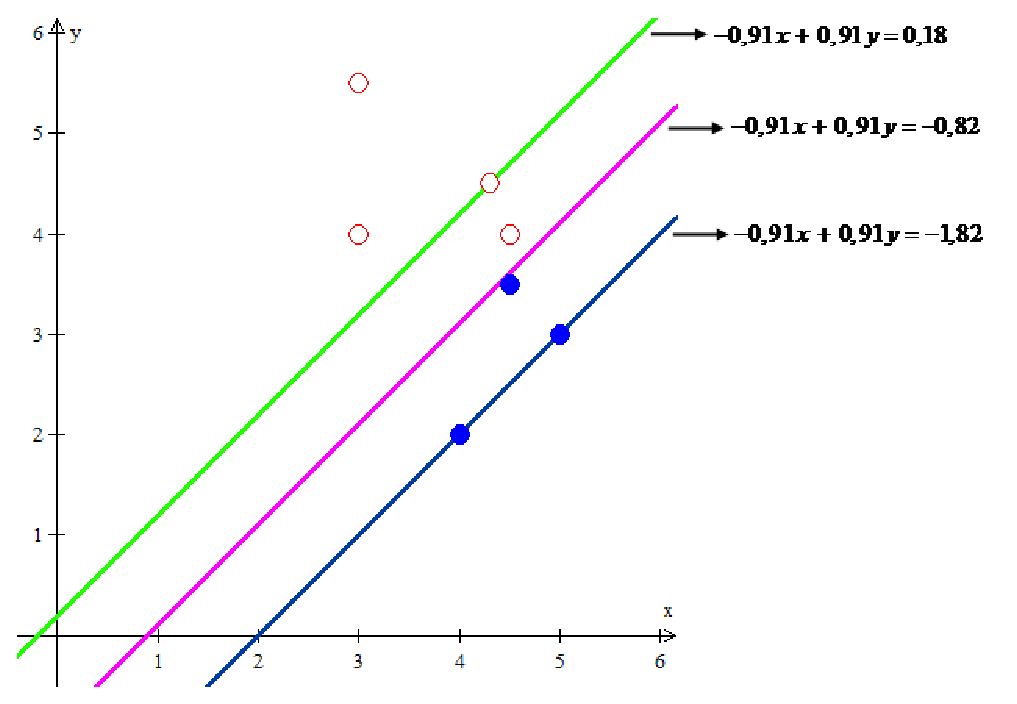
\includegraphics[scale=0.5]{graficos/exemplo1}
	\captionof{figure}{Representação ilustrativa do exemplo 2}
	\label{img:ex2}
\end{center}

Nesse exemplo notamos que o valor 2.46 no vetor y é referente ao ponto do conjunto A que está localizado do lado errado da reta. E o valor 0.91é referente ao ponto do conjunto B que está localizado mais próximo à reta separadora, apesar do ponto estar localizado do ponto correto da reta ele está localizado acima da reta limite $-0.91x + 0.91y = -1.82$.
\end{itemize}

\section{Etapa de classificação}
Após a geração dos classificadores utlizando o modelo de programação linear, é necessário um segundo procedimento onde ocorra de fato classificação de um vetor com padrão inicialmente desconhecido. Nessa etapa de classificação foi implementada uma estrutura de árvore de torneio.
Em seus trabalhos \citeonline{Feng} e \citeonline{Guo} utilizaram a estrutura de árvore de torneio na etapa de classificação após a utilização do modelo de programação linear para gerar os classificadores.
A seguir são apresentadas duas figuras para ilustrar o mecanismo da árvore de torneio.

\begin{center}
	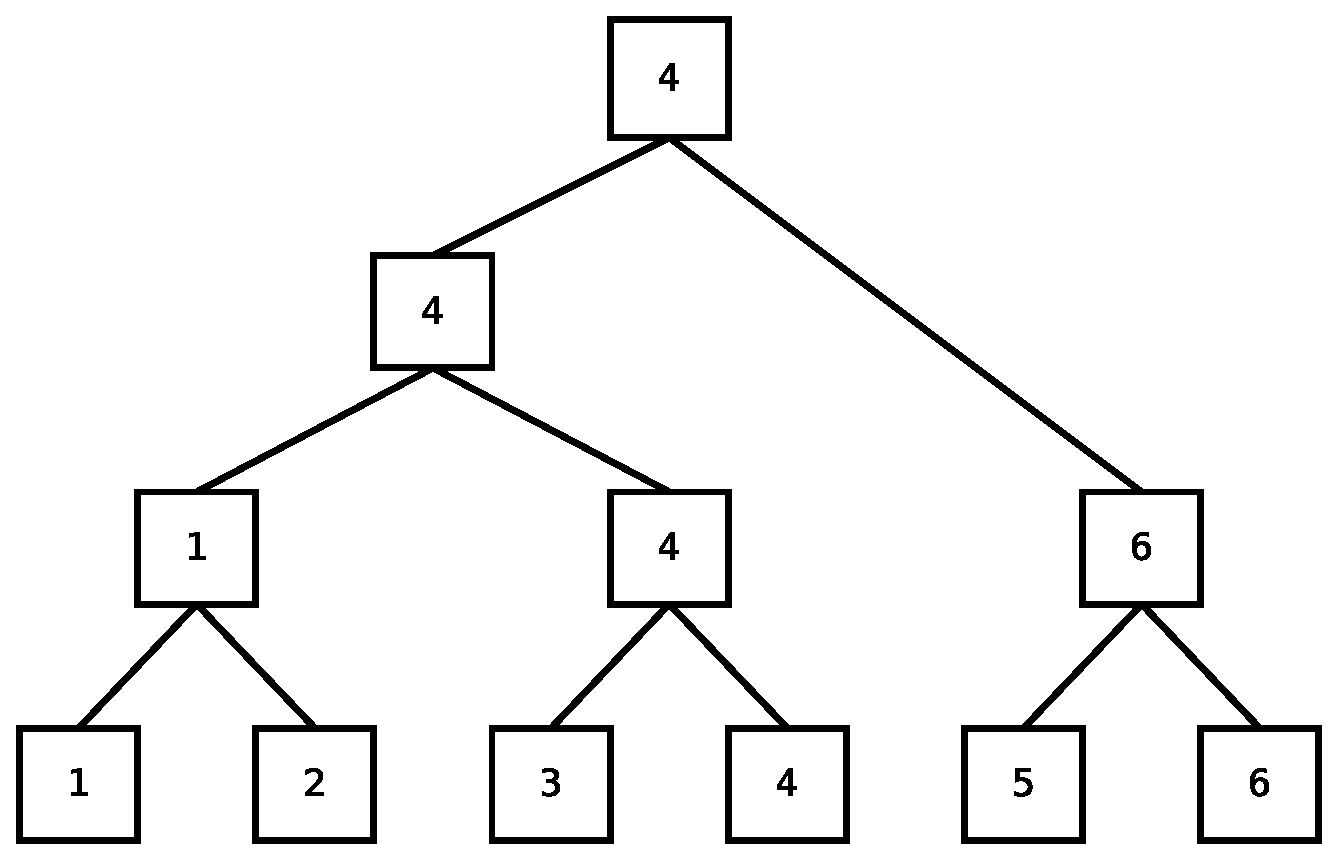
\includegraphics[scale=0.4]{graficos/ArvTorneio1}
	\captionof{figure}{Ilustração de uma árvore de torneio com 6 padrões}
	\label{img:ArvTorneio1}
\end{center}

\begin{center}
	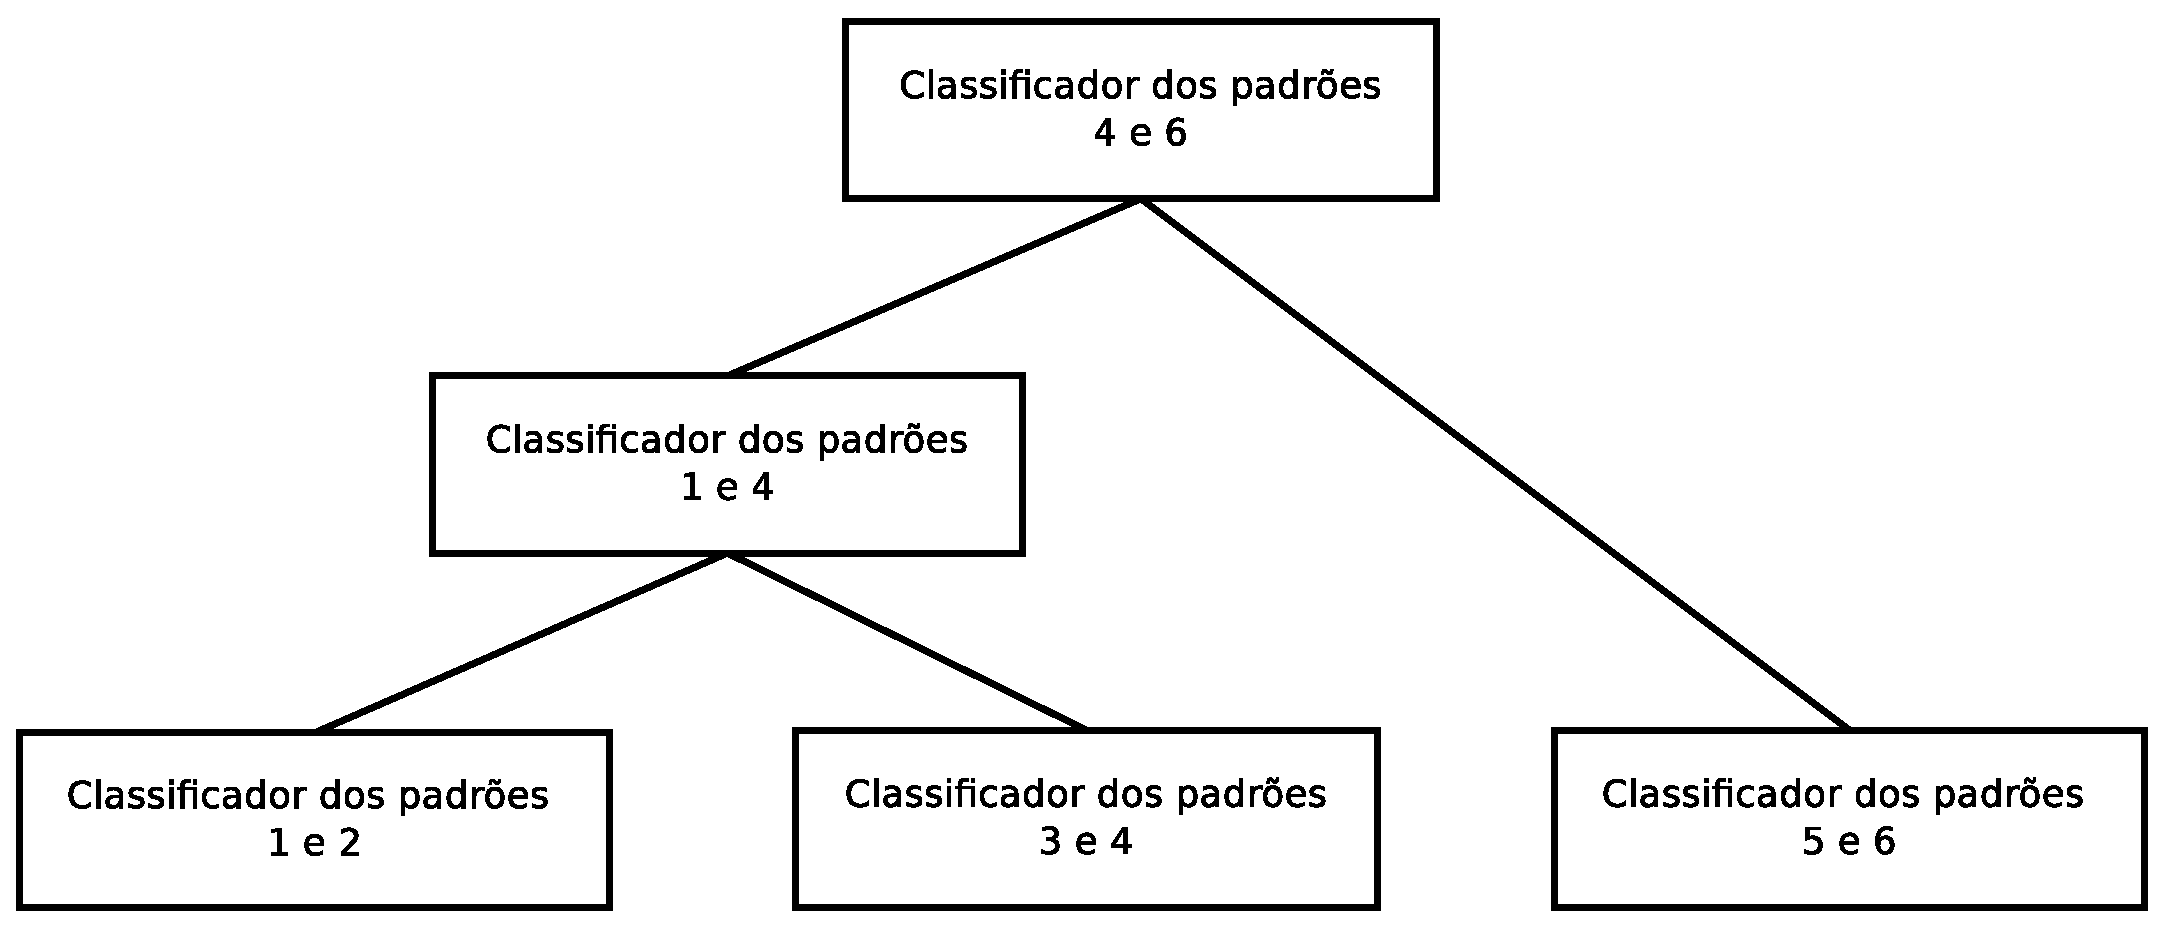
\includegraphics[scale=0.4]{graficos/ArvTorneio2}
	\captionof{figure}{Ilustração de uma árvore de torneio de acordo com os classificadores}
	\label{img:ArvTorneio2}
\end{center}
Depois de obtidos os hiperplanos separadores, é necessário um mecanismo para que um dado com padrão desconhecido possa ser classificado como um dos padrões, ou seja, analisando um vetor é preciso descobrir qual dos padrões ele se classifica. Para isso, é utilizada uma estrutura chamada árvore de torneio \cite{Feng} \cite{Guo}. Por analogia podemos pensar na árvore como a estrutura utilizada em um torneio esportivo e nos padrões como os times do torneio, os times devem se confrontar até que ao final saia o vencedor. Da mesma forma, analisamos os padrões até que ao final se obtenha o padrão ao qual o conjunto submetido pertença.
Na árvore da figura \ref{img:ArvTorneio1}, consideramos 6 padrões e o conjunto desconhecido pertencendo ao padrão 4. A quantidade de nós folhas deve ser a quantidade de padrões e a formação dos pares é arbitrária. Analisando o primeiro par, deve ser analisado em qual dos dois padrões o conjunto desconhecido mais se encaixa, ou seja, deve ser analisado de qual lado da reta (gerada pelo modelo quando foram submetidos os padrões 1 e 2, como ilustrado na figura \ref{img:ArvTorneio2})o conjunto desconhecido se encontra. Na figura exemplo, a maioria dos pontos ficaram localizados do mesmo lado da reta que os pontos do padrão 1, por isso esse padrão continuou no próximo nível da árvore e o padrão 2 foi excluído. Esse procedimento ocorre por analogia em todos os pares, até que ao final, quando analisados os padrões 4 e 6, foi definido que o vetor pertence ao padrão 4.

\chapter{Reconhecimento de Expressões Faciais}

%\section{Introdução}
Segundo \citeonline{FernandoGil} a expressão facial é uma forma de comunicação não-verbal que permite a partilha de
sentimentos e emoções, numa linguagem subentendida entre seres humanos. Desde o início das pesquisas na computação busca-se cada vez mais dotar o computador de um comprtamento inteligente. Sequindo esse caminho, o reconhecimento facial surgiu,  para trazer soluções no campo da Interface Homem- Computador, como um desafio esperado, porém desafiador. Principalmente no reconheciemnto de expressões faciais, já que se trata de um julgamento ambíguo até mesmo para os seres humanos, pois a mesma expressão pode variar de indivíduo para indivíduo \cite{FernandoGil} \cite{Elizabeth}.

\section{Fases do Reconhecimento}
O reconhecimento facial se divide em três etapas básicas \cite{Elizabeth}:
\begin{itemize}
\item Detectar a face na cena: Inicialmente é apresentada uma imagem contendo a face que deve ser rceonhecida. Nesta primeira etapa, deve ser realizada a detecção da zona da face, e devem ser extraídos os outros artefatos que não compõem o rosto \cite{FernandoGil}.
Na figura \ref{img:rosto} é ilustrado o resultado final desta primeira etapa. \\
\begin{center} 
	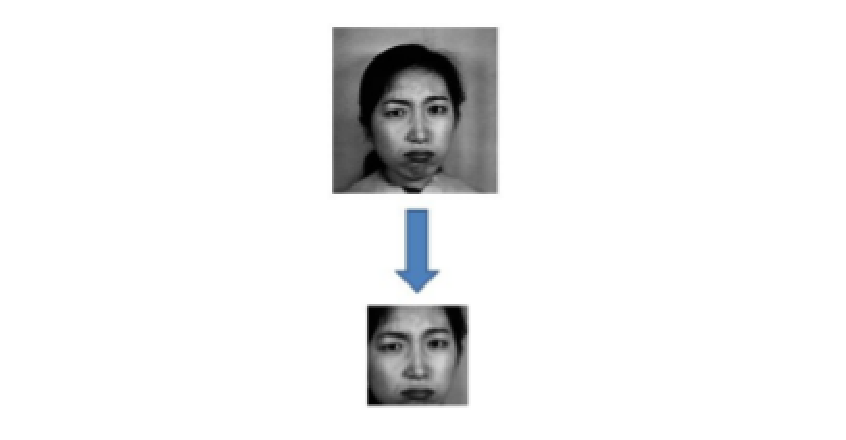
\includegraphics[scale=0.8]{graficos/rosto}
	\captionof{figure}{Detecção da face}
	\label{img:rosto}
	\cite{Elizabeth}
\end{center}
\item Extrair as principais características: Nesta etapa são extraídas as características que são relevantes à classificação da expressão. Normalmente é dada maior ênfase as sobrancelhas, nariz, olhos e boca. \ref{img:rosto_pontos}
A figura abaixo mostra a seleção de pontos mais relevantes para a classificação da expressão. 
\begin{center}
	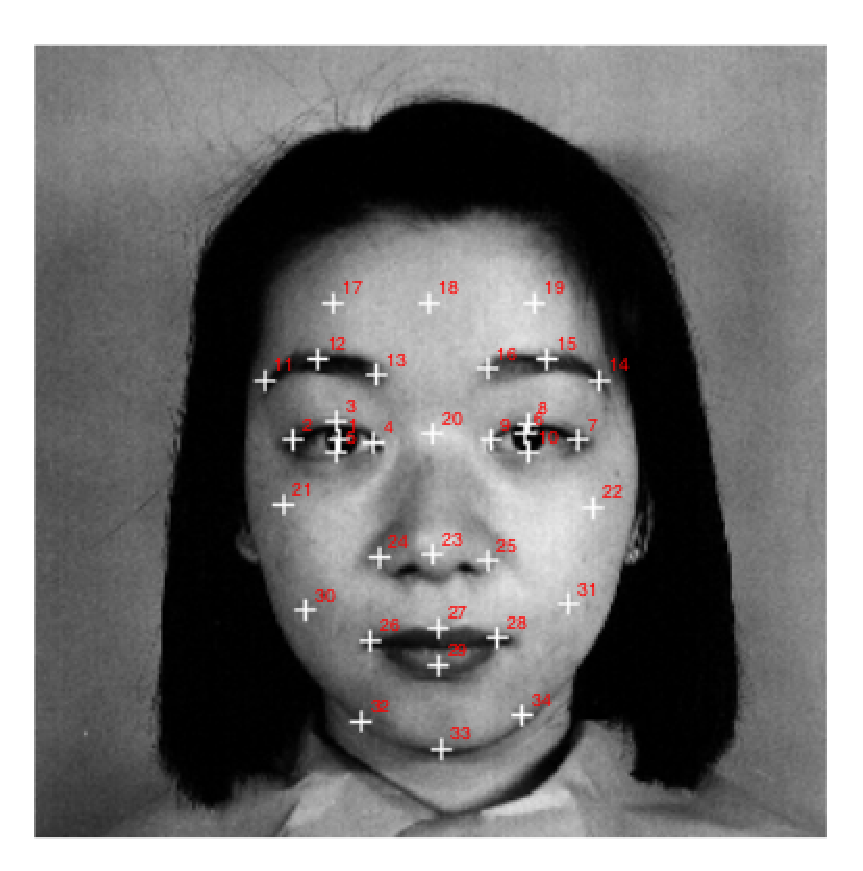
\includegraphics[scale=0.5]{graficos/rosto_pontos}
	\captionof{figure}{Pontos mais relevantes na face}
	\cite{Guo}
	\label{img:rosto_pontos}	
\end{center}
\item Classificar a imagem em uma detreminada expressão: Nesta etapa ocorre de fato a classificação da expressão. Para realizar esta classificação exitem diversos métodos, dos mais simples aos mais complexos. Alguns desse métodos serão apresentados na próxima seção.
\end{itemize} 

Na figura \ref{img:diagrama} está respresentado o processo de reconhecimento facial em suas três etapas básicas. No presente trabalho, a programação linear se aplica na etapa de classificação.
\begin{center}
	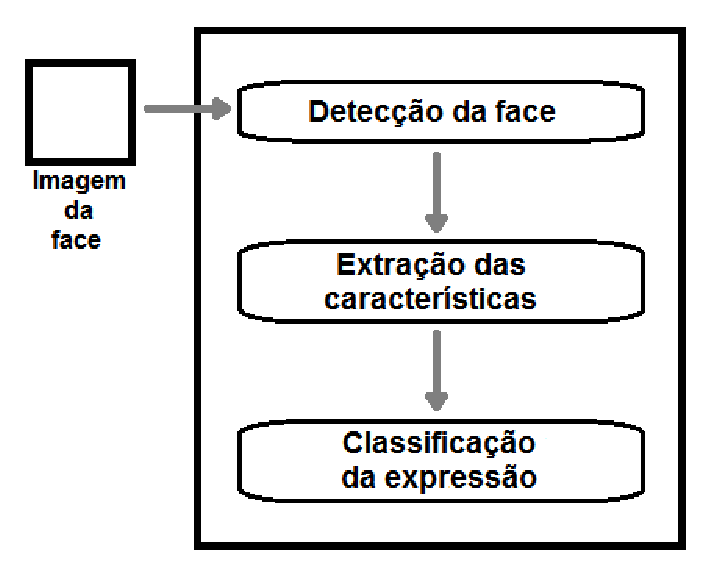
\includegraphics[scale=0.5]{graficos/diagrama}
	\captionof{figure}{Fases do processo de reconhecimento de expressão facial}
	\label{img:diagrama}	
\end{center}

\section{Métodos de Classificação}
Na últipa de etapa do processe de reconheicmento de expressões faciais, é realizada a classificação da expressão. Para a realização desta etapa existem diversos métodos. Alguns deles são apresentados nesta seção. Entre os métodos, existe aquele que utiliza a programação linear, principal fico deste trabalho, e que será apresentado na seção seguinte.

Em \cite{Hong} é descrito um método onde é utlizada uma base de dados com imagens de diferentes indivíduos relativas às expressões. A face a ser classificada é associada a face mais semelhante dentre as existentes na base dados, e após isso a expressão é classificada. Este método parte do princípio que pessoas com fisionomias semelhantes possuem uma maneira similar de apesentar a mesma expressão. Através de uma estrtura denominada General Face Knowledge são criados grafos sobre as imagens, através de pontos-chave da face. Quando o grafo do rosto, a ter sua expressão reconhecida, é criado, este é comparado aos grafos das imagens da base de dados, para que uma face semelhante seja encontrada. Na figura \ref{img:metodo1_classi} é ilustrado uma grfao sobre uma face. Esta abordagem obteve uma taxa de sucesso de cerca de 89\%.
\begin{center}
	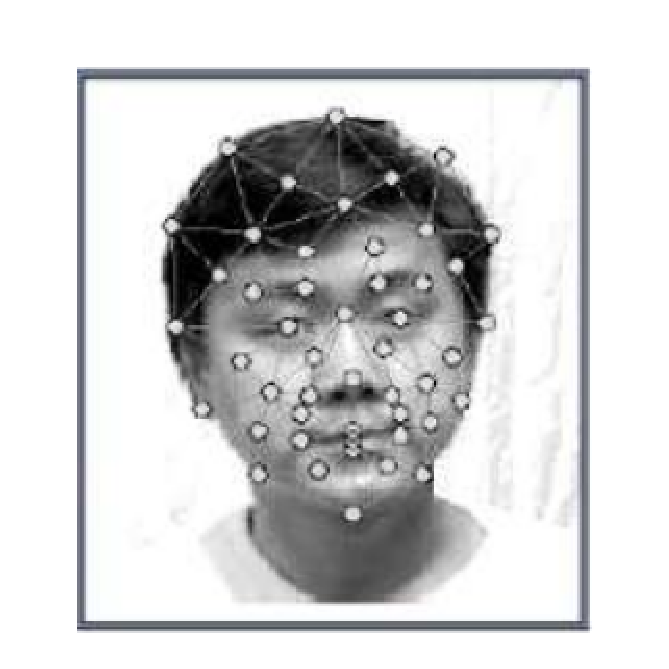
\includegraphics[scale=0.5]{graficos/metodo1_classi}
	\captionof{figure}{Exemplo de aplicação de General Face Knowledge ao rosto}
	\label{img:metodo1_classi}
\end{center}

\cite{Edwards} apresenta um outro método, em que é utilizado um framework denominado Active Appearance Models, nessa abordagem o objetivo é detectar a face idependente da luminosidade e posição. O  Active Appearance Models
possui um modelo estático que deve se ajustar a face que está sendo analisada através de alguns parâmetros e de forma iterativa. A figura \ref{img:metodo2_classi} ilustra o método.
\begin{center}
	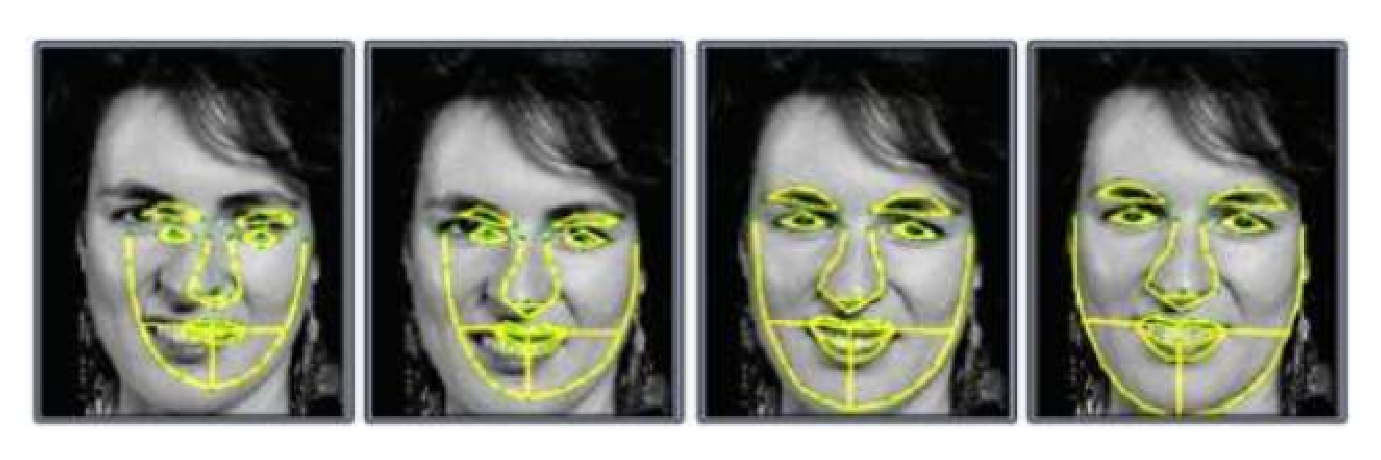
\includegraphics[scale=0.5]{graficos/metodo2_classi}
	\captionof{figure}{Ajuste do Active Appearence Models em três iterações a partir da posição inicial}
	\label{img:metodo2_classi}
\end{center}

Em um outro trabalho são definidas características-modelo, que são comparadas às características da face neutra, ou seja, sem expressar emoção, do indivíduo que está sendo analisado. Após essa etapa, é analisada a deformação, em relação ao modelo, quando o indivíduo expressa alguma emoção. A partir da deformação é realizada a classificação da expressão. A taxa de sucesso é de 92\% para a metade superior da face e de
86\% para a metade inferior. Na imagem \ref{img:metodo3_classi} é ilustrado o ajustamento das características modelo ao olho \cite{Pantic}.
\begin{center}
	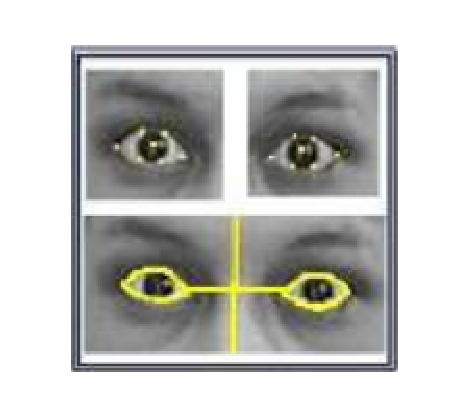
\includegraphics[scale=0.5]{graficos/metodo3_classi}
	\captionof{figure}{ Ajustamento ao olho: características-modelo}
	\label{img:metodo3_classi}
\end{center}

\section{O Reconhecimento de Expressões Faciais e a Programação Linear}

Em seus trabalhos, \citeonline{Feng} e \citeonline{Guo} apresentaram uma abordagem de reconhecimento de expresssões faciais utilizando a programação linear. Em ambos a programação linear foi utilizada na fase de classificação da expressão. Em \citeonline{Guo} a programação lienar foi utlizada ainda na fase de extração de carcaterísticas, para determinar a quantidade de caracteríticas a serem selecionadas e os principais pontos da face. Enquanto no trabalho de \cite{Feng} é utilizado o filtro de Gabor na etapa de extração de carcaterísticas. O Filtro de Gabor tem a capacidade de realçar bordas e saliências na imagem. Após a aplicação do filtro na imagem, são realçadas as características salientes presentes no rosto (cantos dos olhos, cantos da boca, narinas, entre outros) \cite{Gabor}. Em ambos os trabalhos foram obtidos ótimos resultados e superiores a outros métodos com os quais foram comparados. 

A programação linear é utlizada na etapa após o tratamento da imagem. Primeiramente as expressões são combinadas em pares. No trabalho de \cite{Feng}, por exemplo, busca-se o reconhecimento de sete expressões: raiva, desgosto, medo, felicidade, tristeza, surpresa e neutro. Essas expressões são combinada em pares do tipo: raiva-desgosto, raiva-medo, etc. Formando um total de 21 pares. Após isso o modelo de programação linear, apresentado mais adiante, é utilizado para gerar os calssificares, o modelo deve ser rodado 21 vezes, uma para cada par de expressões. Essa etapa é também chamada de treinamento, pois a partir do classificadores gerados as expressões das imagens a serem analisadas serão determinadas. Essa abordagem também substitui a utilização de redes neurais para o treinamento, uma vantagem é que o modelo necessita ser rodado uma única vez para cada par, enquanto em uma abordagem utilizando redes neurais este processo se trona iterativo.

$Min\ \frac{e^{t}y}{m} + \frac{e^{t}z}{k}\\
\ subject\ to  \\
\              -A\omega + e\gamma + e <= y\\
\              B\omega - e\gamma + e <= z\\
\              y>= 0, z>= 0 $

Onde, 
\begin{itemize}
\item \textbf {$m$} representa a quantidade de imagens de rostos com a primeira expressão do par
\item \textbf {$k$} representa a quantidade de imagens de rostos com a segunda expressão do par
\item \textbf {$e$} é um vetor de 1's
\item \textbf {$y$} e {$z$} são as varáveis do modelo
\item \textbf {$A$} é a matriz de pontos das imagens de rostos com a primeira expressão do par
\item \textbf {$B$} é a matriz de pontos das imagens de rostos com a segunda expressão do par
\end{itemize}

Na última etapa de determinação da exepressão é utilizda uma estrtura de árvore binária de torneio.

Através dessa arbordagem espera-se comprovar os ótimos resultados mostrados pelos trabalhos que utilizam a programação linear.


%--------------------------------- Bibliografia --------------------------------

\citeoption{abnt-repeated-author-omit=yes}
\bibliographystyle{abnt-alf}
\bibliography{bibliografia}

\end{document}

